Lors de ce projet de fin d’étude notre organisation s’est divisé en deux partie : 
\begin{itemize}
    \item Avant Projet XL 
    \item Projet XL 
\end{itemize}

\section{Avant Projet XL}

\subsection{Objectif SMART}
Afin de mieux délimiter le projet et ses objectifs, nous avons convenu avec le client d'un certain nombre d'objectifs, correspondant au critères SMART. Ces objectifs de projet nous ont permis de mieux juger de la charge de travail nécessaire et nous a donné des buts à atteindre. Nous étions donc également en mesure de pouvoir quantifier l'avancement du projet. Ces objectifs étaient : 

\begin{itemize}
    \item Construire un système d'extraction du texte brut depuis des PDF  
    \item Extraire une liste de métadonnées (définie par le client) depuis le texte brut
    \item Assigner au moins une taxonomie au texte 
    \item Indexer les documents de notre base de données à partir des informations extraites (métadonnées et taxonomies)
    \item Interfaçage avec un moteur de recherche  
\end{itemize}

Nous étions capables de vérifier si chacun de ces objectifs était accomplis grâce à une série de test, définie section 8 du DER. 



\subsection{Gantt}
Dans un premier temps, nous avions effectué un planning de Gantt post mortem avec les grandes tâches. Cette étape a été l’une de nos premières tâches. Cette organisation permet d’avoir une estimation de la charge de travail. 
Avec la complexité du projet, nous voulions nous consacrer sur les tâches les plus importantes. Cependant, il valait mieux avoir un diagramme général afin d’avoir un support visuel pour évaluer la charge de travail restante. 

\begin{figure}[h!]
  \centering
  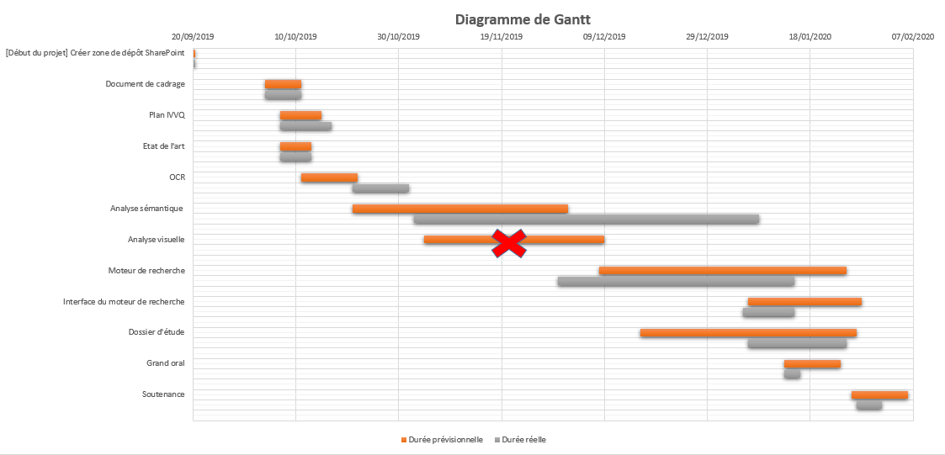
\includegraphics[width=0.8\textwidth]{DiagrammeGanttAvantXL.png}
	\caption[]{Diagramme de Gantt post moderm}
	\label{}
\end{figure}

Le schéma ci-dessus est le diagramme de Gantt qui nous a permis de nous aiguiller tout le long du projet. En orange nous avons la durée des tâches que nous avons estimées et en gris leurs durées réelles.
Nous pouvons remarquer que nous sommes généralement dans les temps même si certaines tâches ont pris plus de temps que prévues. L’analyse sémantique représente la taxonomie qui est la charge de travail la plus importantes. 
L’analyse visuel nécessaire a été supprimé en cours de route car suite à une réunion avec le commanditaire, il nous a été demandé de centrer le POC sur un seul type de document. De ce fait, nous avons gagné plus de temps pour nous focaliser sur d’autres tâches. 



\subsection{Gantt Hebdo}
Le diagramme représenté dans la partie 12.2) est très bien pour avoir une vue globale sur l’avancement du projet. Cependant, pour chaque grande tâche dépendent des tâches plus petites. 
C’est la raison pour laquelle nous avons fait un diagramme hebdomadaire divisé en sept sprints. 

\begin{figure}[h!]
  \centering
  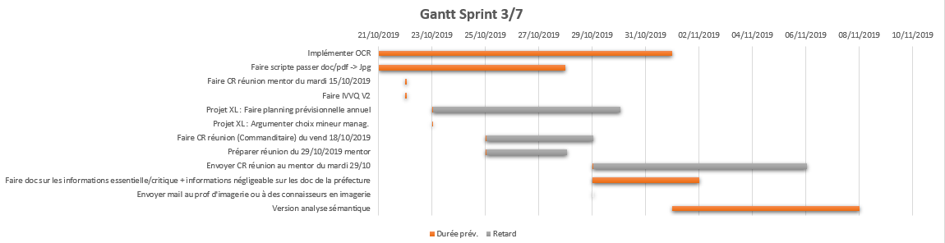
\includegraphics[width=0.8\textwidth]{DiagrammeGanttHebdoAvantXL.png}
	\caption[]{Diagramme de Gantt hebdomadaire sprint 3/7}
	\label{}
\end{figure}

Cette démarche nous a été d’une grande aide afin de nous guider sur notre avancement. Ci-dessus, nous avons l’exemple du sprint 3/7 qui concerne en partie de notre demande de projet XL et l’implémentation d’une OCR. 
Nous avons des indications sur la durée que nous avons prévu (en orange) et le retard que nous avons pris (en gris). 



\subsection{Organisation}
Deux membres de l’équipes travaillaient depuis Laval et l'autre depuis Paris. Cela ne nous a pas dérangé, cette situation nous a permis d’organiser des réunions régulières avec le commanditaire. 

\subsubsection{Sharepoint et Github}
Afin de nous organiser, l’ensemble des fichiers non-techniques étaient stockés sur le Sharepoint Cap Projet. Ce dernier se compose des documents administratifs, de nos comptes rendus de réunions, des recueils administratifs de la préfecture et d’un trombinoscope. 
Il nous permet de nous structurer et d’informer notre mentor lorsqu’un document est disponible. 

En ce qui concerne de nos programmes, nous avons fait le choix de travailler avec Github qui est un service web d'hébergement et de gestion de développement de logiciels. Ainsi, nous avions un contrôle de version des codes développés. 


\subsubsection{Réunions}
Pour un suivi régulier du projet, nous faisions une réunion par semaine avec notre mentor. Avec la distance de travail entre les membres de l’équipe et le mentor (Paris-Laval), nous communiquions en visioconférence. 
C’est avec des PowerPoints que nous présentions notre avancement. Cette démarche a permis d’avoir une réunion structurée, lisible et présentable. 

\begin{figure}[h!]
  \centering
  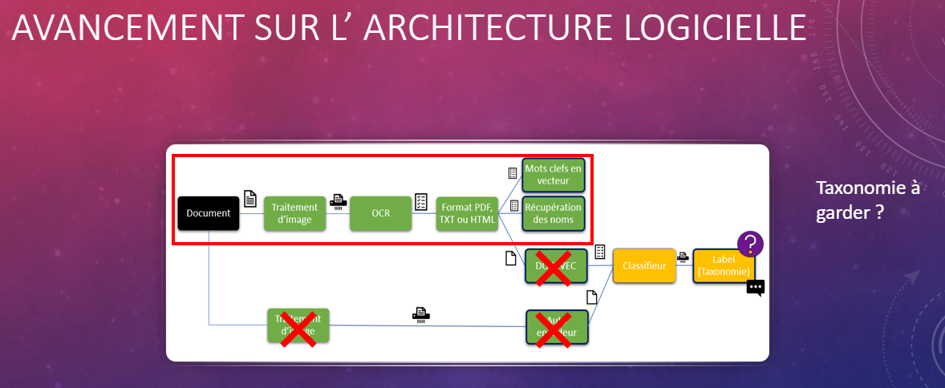
\includegraphics[width=0.8\textwidth]{ArchitecureLogicielAvantXL.png}
	\caption[]{Avancement architecture logiciel}
	\label{}
\end{figure}




\subsection{Charge de travail}
Au début du projet, nous avions accès à un fichier Excel sur le SharePoint. Dans un premier temps, nous avions évalué les charges de travail qui seront nécessaire pour chaque tâche. Cette démarche nous a permis de réaliser l’ampleur de ce projet et par la suite de faire une demande de projet XL. 
Nous avons établi la charge prévisionnelle suivante :

\begin{figure}[h!]
  \centering
  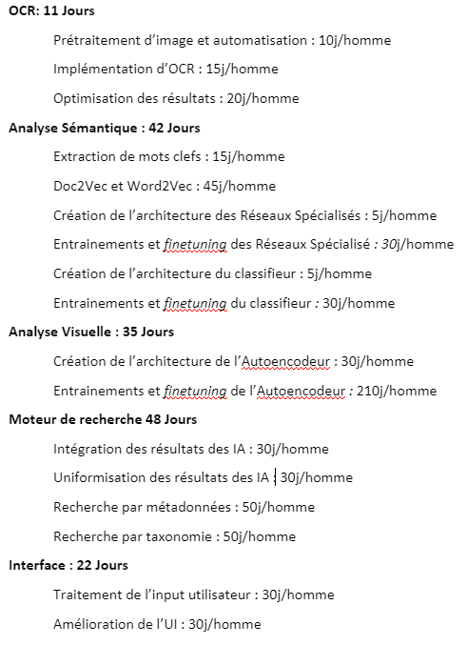
\includegraphics[width=0.8\textwidth]{ChargeDeTravailAvantXL.png}
	\caption[]{Charge de travail prévisionnel}
	\label{}
\end{figure}

Nous remarquons que nous avons pris de la marge sur l’évaluation des tâches en jours/hommes à cause des différents risques que nous pourrions rencontrer. La charge de travail réel est deux fois moins que ce que nous avons évalué. 
En réalité, nous avons effectué une charge de travail équivalent à 504 heures.





\section{Projet XL}

\subsection{Organisation}
Suite à l’évaluation des charges de travails que nous avions besoin pour terminer le projet, nous avions fait une demande de projet XL qui consiste à remplacer nos heures de mineurs managériales par la réalisation de notre PFE. 
Ce projet XL aura duré trois semaines 06/01/2020 – 24/01/2020. Dans un premier temps, nous avons jugé qu’il serait plus intéressant de commencer par revoir notre organisation. Il faut que chaque jour, nous avancions sur une tâche et que nous voyons l’avancement du projet. C’est la raison pour laquelle nous avons décidé d’appliquer au mieux la méthode agile Scrum.
Après avoir listé l’ensemble des tâches, nous les avons divisés en deux sprints :

\begin{itemize}
    \item Sprint 1 : Version 1 PoC. Semaine 06/01/2020 – 10/01/2020 
    \item Sprint 2 : Version 2 PoC et DER. Semaine 13/01/2020 - 05/02/2020
\end{itemize}

Le sprint 2 a une durée plus élevée que le premier sprint dû à la différente charge de travail. Il correspond en partie aux tâches non techniques (DER, Grand Oral et Soutenance). 
Comme outil, nous avons utilisé Trello qui est un outil de gestion de projet.  


\subsection{Trello}
Trello est un outil de gestion de projet en ligne, lancé en septembre 2011 et inspiré par la méthode Kanban de Toyota. Il repose sur une organisation des projets en planches listant des cartes, chacune représentant des tâches. 
Durant le projet XL, nous avons utilisé cet outil pour sa visualisation et son efficacité avec les méthodes agiles. 
Pour mieux s’organiser, nous avons divisé les tâches en six parties ayant chacun un code couleur : 

\begin{itemize}
    \item Métadonnées (bleu ciel): Sprint 1 
    \item Taxonomie (bleu foncé): Sprint 1 
    \item Moteur de recherche: Sprint 1 et 2 
        \begin{itemize}
            \item Ajout Json
            \item Interface
        \end{itemize}
    \item DER: Sprint 2
    \item Grand Oral: Sprint 2  
    \item Soutenance: Sprint 2 
\end{itemize}


\begin{figure}[h!]
  \centering
  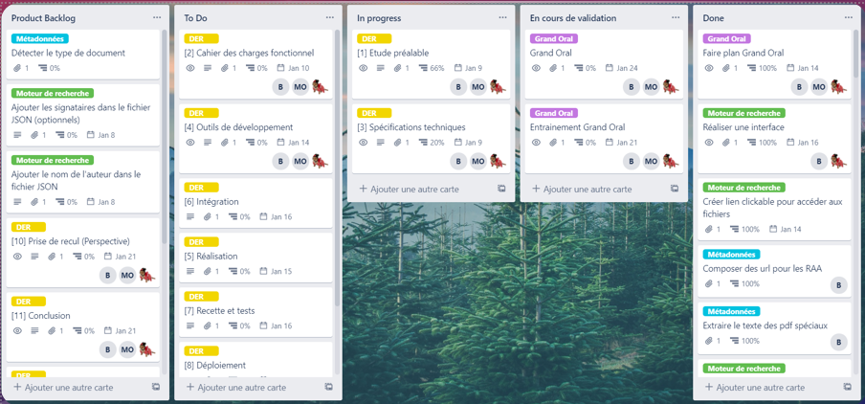
\includegraphics[width=0.8\textwidth]{ScrumBoardXL.png}
	\caption[]{Scrum board dans Trello}
	\label{}
\end{figure}

Ce tableau de bord du projet est accessible et visible en permanence de l’ensemble de l’équipe projet. Il va permettre de suivre en temps réel l’évolution des tâches et des user stories à réaliser. Le scrum board est séparé au minimum en trois parties : Le product backlog, les tâches à faire, les tâches en cours et les tâches terminées.
Nous avons ajouté une phase « En cours de validation » afin de vérifier que les tâches ont bien été faite. 


\subsection{Scrum}
La méthode agile permet de délivrer un projet/produit très rapidement. Ce cadre méthodologique est conçu sur des cycles de développement court durant lesquels on s’adapte constamment tout maintenant l’utilisateur au centre. 
Elle se compose de :

\begin{itemize}
    \item Scrum master 
    \item Product Owner 
    \item Développer(s) 
\end{itemize}

Le scrum master est garant du processus scrum. Il s’assure d’une bonne communication entre les membres de l’équipe. Afin que l’équipe comprenne bien cette méthodologie de travaille, le scrum master a écrit un document qui l’explique en détail.
De plus elle se compose aussi d’un product owner qui représente le client. Il définit les spécifications fonctionnels (ex :  document Integration Validation Verification Qualification) et établie la liste des priorités de ce qu’il faut développer. C’est aussi lui qui valide les fonctionnalités.



\subsubsection{User Story}
Le processus Scrum commence par le user story. Il décrit l’expérience utilisateur en utilisant le langage, le vocabulaire et la terminologie de l’usager.   
Chaque user story comporte : 

\begin{itemize}
    \item Un identifiant : un nom contenant la fonction du produit de manière succincte  
    \item L’importance : Une valeur qui définit la priorité de la story  
    \item Estimation du travail nécessaire
    \item Démonstration : Un test simple de la story qui sera à valider   
\end{itemize}

Nous avons décrit l’ensemble des exigences du commanditaire en user story de la manière suivante : 

\begin{figure}[h!]
  \centering
  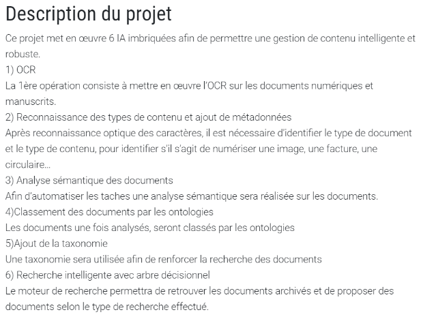
\includegraphics[width=0.8\textwidth]{DescriptionProjetXL.png}
	\caption[]{Description du projet}
	\label{}
\end{figure}

\begin{figure}[h!]
  \centering
  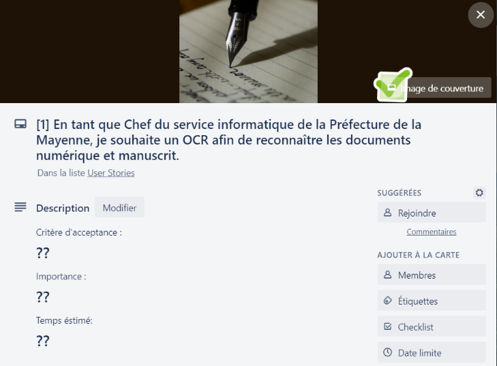
\includegraphics[width=0.8\textwidth]{userStoryXL.png}
	\caption[]{Exemple d’un user story}
	\label{}
\end{figure}

Cette étape nous a permis de nous recontextualiser le PoC demandé par le commanditaire. 


\subsubsection{Product backlog}
De la user story va émaner des exigences. Elles seront hiérarchisées avec le client dans un product backlog. Nous pouvons le voir comme un carnet de commande pour le produit. C’est un miroir de ce qu’il faut faire pour réaliser les besoins du client et délivrée la user story.  
Le product backlog va constamment évoluer pour refléter les nouveaux besoins. 
En listant l’ensemble des taches dans un document word, nous avons pu catégoriser l’ensemble des tâches.

\begin{figure}[h!]
  \centering
  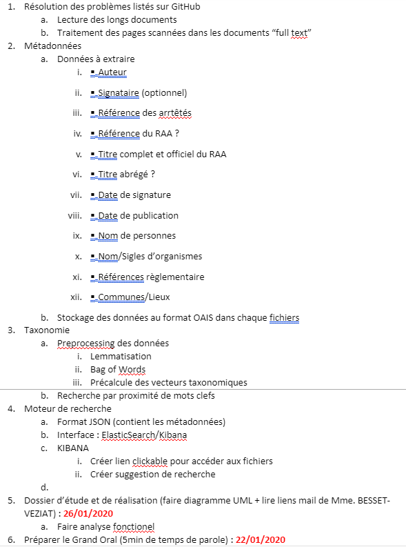
\includegraphics[width=0.8\textwidth]{ListePrevisionnelleXL.png}
	\caption[]{Liste prévisionnelle des taches}
	\label{}
\end{figure}

\begin{figure}[h!]
  \centering
  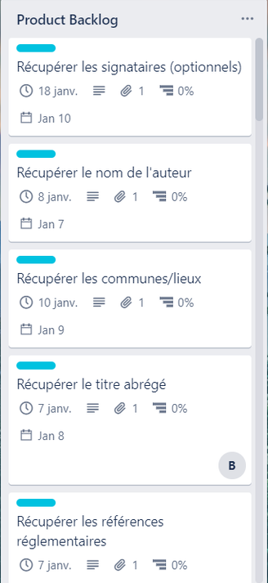
\includegraphics[width=0.8\textwidth]{ProductBacklogXL.png}
	\caption[]{Product backlog sous trello}
	\label{}
\end{figure}



\subsubsection{Sprint}
Une fois d’accord avec la user story et les exigences (product backlog), il est temps de se lancer dans la réalisation du projet. Il sera découpé en plusieurs itérations que l’on nomme des sprints. 
Les étapes du sprint sont :

\begin{itemize}
    \item Sprint planning meeting:Un sprint commence par une réunion de planification. Au cours de cette séance, on va aller puiser les éléments prioritaires du product backlog qui seront développés dans les sprints.  Aussi nommé daily meeting, nous avons utilisé cette méthode. Nous avions réunions du tous les matins à partir de 10h (lundi-vendredi) afin d’attribuer les tâches de la journée. Nous avons rajouté une autre réunion le soir à partir de 19h qui n’est pas prévu dans la méthode Scrum. Cette dernière réunion nous a permis de revoir les difficultés que nous avons rencontré et de discuter des tâches de la journée. 
    \item Sprint backlog : Dans chaque sprint qui durent entre 2-4 semaines, il y aura du développement puis un contrôle qualité (du test) et une livraison. L’ensemble des livraisons des sprints cumulé se nomment le sprint backlog. C’est la réunion avec le commanditaire par équivalence. Cela nous a permis de proposer deux versions de PoC.   
\end{itemize}

\subsection{Horaires}
Nos horaires de travails étaient en moyenne de 10h – 18h avec une pause déjeuner vers 12h.
Nous avions une réunion tous les matins à partir de 10h et un le soir à partir de 19h.



\subsection{Charge de travail}

Prévisionnel : 

En listant l’ensemble de tâches, nous avons établi leurs charges de travail en jours/hommes et en heures. 
Nous avons donc les tâches suivantes : 

\begin{itemize}
    \item Sprint 1 (06/01/2020 – 10/01/2020) :
        \begin{itemize}
            \item Métadonnées : 6 jours/hommes pour 2 personnes
            \item Taxonomie : 18 jours/hommes our1 personnes
            \item Moteur de recherche : 15 jours/hommes 2 personnes
        \end{itemize}
    \item Sprint 2 (13/01/2020 - 03/02/2020) :
    \begin{itemize}
        \item DER : 11 jours/hommes pour 3 personnes
        \item Grand Oral : 6 jours/hommes pour 3 personnes
        \item Soutenance :  9 jours/hommes pour 3 personnes
    \end{itemize}
\end{itemize} 

Total :  Nous avons prévu un total de 65 jours/hommes de travail en 3 semaines pour 3 personnes.


Réel : 

\begin{itemize}
    \item Sprint 1 (06/01/2020 – 10/01/2020) :
        \begin{itemize}
            \item Métadonnées : 9 jours/hommes pour 2 personnes
            \item Taxonomie : 12 jours/hommes our1 personnes
            \item Moteur de recherche : 31 jours/hommes 2 personnes
        \end{itemize}
    \item Sprint 2 (13/01/2020 - 03/02/2020) :
    \begin{itemize}
        \item DER : 58 jours/hommes pour 3 personnes
        \item Grand Oral : 8 jours/hommes pour 3 personnes
        \item Soutenance :  9 jours/hommes pour 3 personnes
    \end{itemize}
\end{itemize} 

Total :  Nous avons effectué un total de 127 jours/hommes en 3 semaines pour 3 personnes.

Ci-dessous nous pouvons voir la comparaison des charges de travail réel contre ce dont nous avons prévu en jours/hommes : 

\begin{figure}[h!]
  \centering
  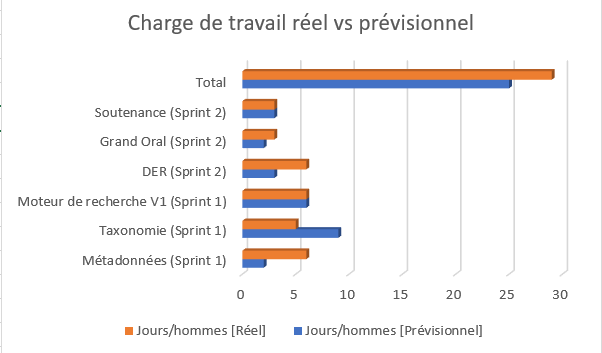
\includegraphics[width=0.8\textwidth]{ChargeTravailXL.png}
	\caption[]{Charge de travail prévisionnel contre réel en jours/hommes}
	\label{}
\end{figure}



\subsection{Gantt prévisionnel/réel}
Au début du projet XL, nous avons effectué un diagramme de Gantt prévisionnel afin de comparer les charges de travails ainsi que la durée de chacune des taches. Le diagramme du projet XL commence le 06/01/2020 et se termine le 05/02/2020. 
Sur l’image ci-dessous, nous avons listé certaines taches datant du 02/12/2019 nous avons quelques dépendances pour les taches du début du projet XL. De plus, on peut remarquer que nous avons des indications de pourcentage pour le projet et les taches. Dans notre Trello, lorsqu’une tâche est dans le product backlog ou dans la section “To do” elle est automatiquement à 0 pourcent. En passant dans “In progress” elle passe à 20 pourcent, dans “En cours de validation” à 80 pourcent puis à 100 pourcent lorsqu’elle est dans “Done”. Ainsi nous avions un diagramme dynamique avec une métrique plus intéressante comparé à notre ancien Gantt. Ci-dessous nous avons le diagramme de gantt prévisionnel et réel : 

\begin{figure}[h!]
  \centering
  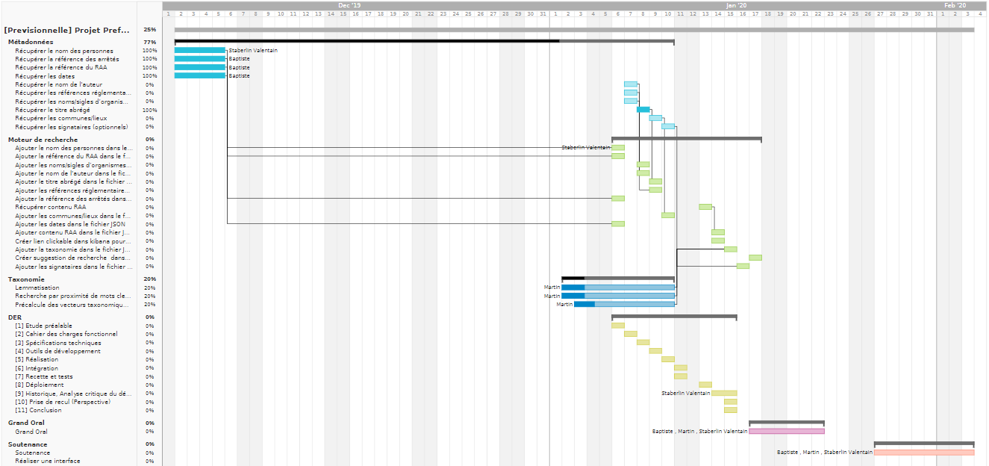
\includegraphics[width=0.8\textwidth]{GanttPrevisionnelXL.png}
	\caption[]{Digramme de Gantt Projet XL prévisionnel}
	\label{}
\end{figure}

\begin{figure}[h!]
  \centering
  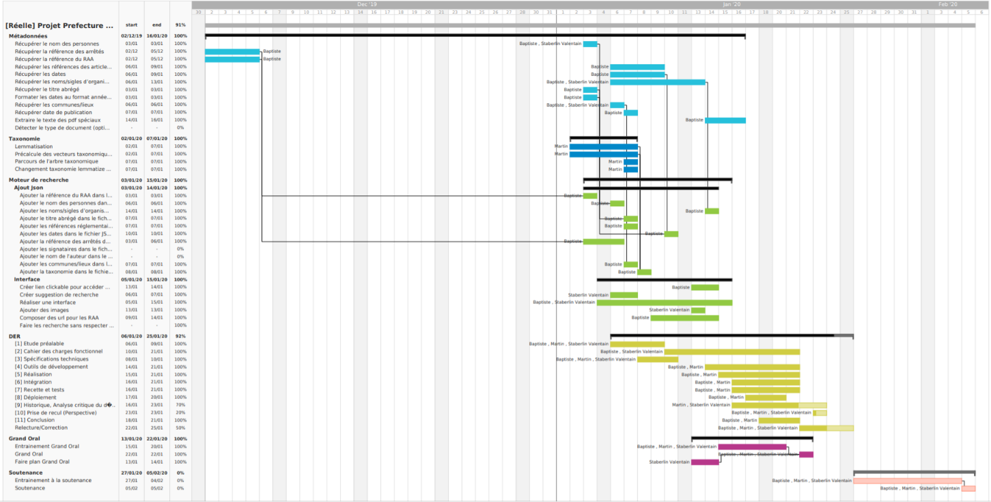
\includegraphics[width=0.8\textwidth]{GanttReelXL.png}
	\caption[]{Digramme de Gantt Projet XL réel}
	\label{}
\end{figure}


\subsubsection{Sprint 1 Réel/prévisionnel (Gantt Hebdo)}
A l’aide de Trello, nous avions établi un calendrier hebdomadaire. Ce dernier nous a permis d’avoir une indication visuelle sur le nombre de tâches que nous avons par jours. Si nous devions comparer les deux images ci-dessous (prévisionnel et réel), nous pouvons remarquer que certaines tâches ont pris moins de temps que prévues. Cependant, la quantité de travails par jours est plus importantes.

\begin{figure}[h!]
  \centering
  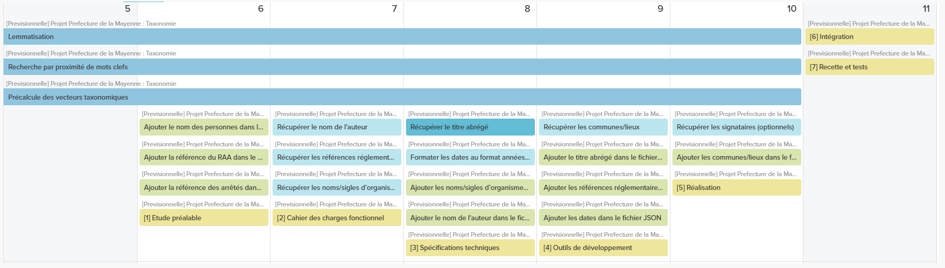
\includegraphics[width=0.8\textwidth]{GanttPrevHebdoSprint1XL.png}
	\caption[]{Calendrier prévisionnel Sprint 1 (06/01/2020 - 10/01/2020)}
	\label{}
\end{figure}

\begin{figure}[h!]
  \centering
  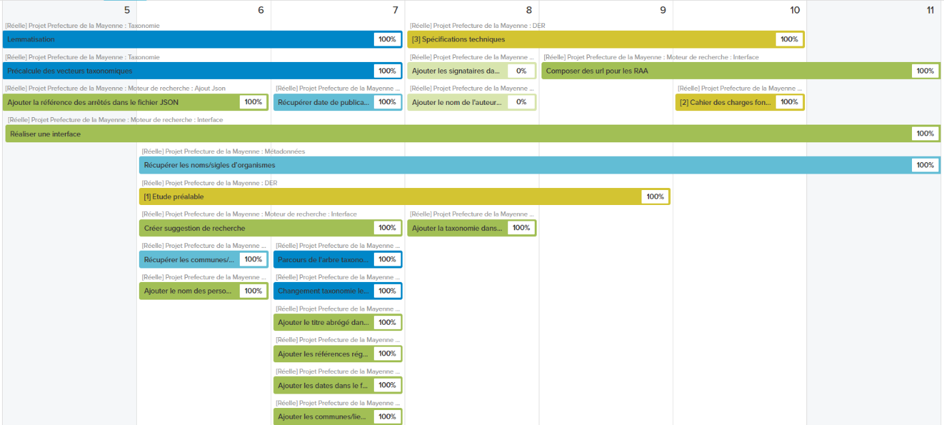
\includegraphics[width=0.8\textwidth]{GanttReelHebdoSprint1XL.png}
	\caption[]{Calendrier réel Sprint 1 (06/01/2020 - 10/01/2020)}
	\label{}
\end{figure}



\subsubsection{Sprint 2 Réel/prévisionnel (Gantt Hebdo)}
Le deuxième sprint est plutôt consacré au DER, au Grand Oral ainsi qu’à la soutenance. Nous n’avons pas prévu que le DER aurait pris autant de temps (visible sur les images ci-dessous). Comme résultat, nous nous sommes retrouvés a effectué plus de tâches que prévues par jours. 

\begin{figure}[h!]
  \centering
  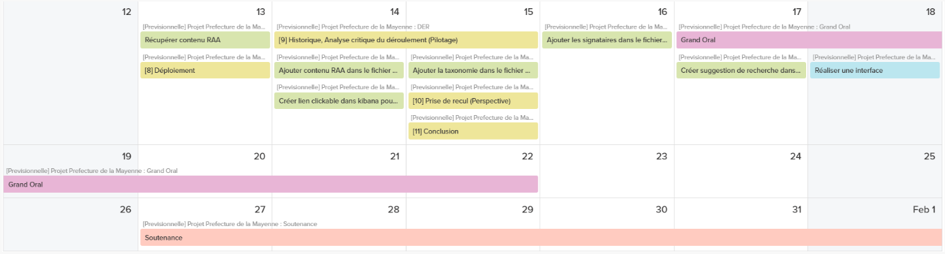
\includegraphics[width=0.8\textwidth]{GanttPrevHebdoSprint2XL.png}
	\caption[]{Calendrier prévisionnel Sprint 2 (13/01/2020 - 05/02/2020)}
	\label{}
\end{figure}

\begin{figure}[h!]
  \centering
  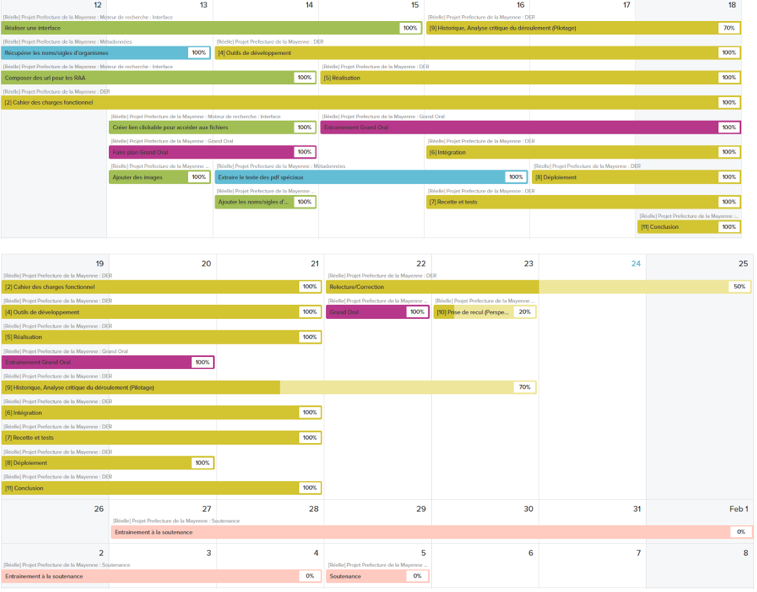
\includegraphics[width=0.8\textwidth]{GanttReelHebdoSprint2XL.png}
	\caption[]{Calendrier réel Sprint 2 (13/01/2020 - 05/02/2020)}
	\label{}
\end{figure}

Même si le diagramme de gantt n'a pas été respecté tel que prévu, le fait d’avoir estimé les charges de travails ainsi que d’établir un calendrier de travail cela nous a permis d’être à temps sur l’ensemble du projet. Nous pouvons en déduire que la méthode agile a accéléré l’avancement du projet.